\FloatBarrier
\section{Dense Pulse-Length Dependence}
\label{sec:dense-pulse-length}

\subsection{Acquisition and campaign-specific normalization}

A separate q6 campaign on September 9--10, 2026 tests the dependence on the
pulse duration $L$ at fixed relative cutoff $c=0.005$. Each duration
$L=1,2,5,10,15,20,25,30,35,$ and $40~\mu\mathrm{s}$ was acquired once,
using 400 uniformly spaced detunings over $[-1,1]~\mathrm{MHz}$ and 400
logarithmically spaced nominal amplitudes from $0.01$ to $0.70~\mathrm{V}$,
with 380 averages per grid point. The waveform template duration equals
$L$, with no duration stretching. The echo has an abrupt midpoint sign
reversal; the derivative quadrature is disabled ($\beta=0$), and no
AC-Stark compensation is applied (effective $\kappa=0$). The finite envelope
therefore changes its time scale together with $L$, rather than varying the
truncation time of a fixed-width pulse.

The saved square-$\pi$ calibration is $t_\pi=40~\mathrm{ns}$ at
$A_\pi=0.203776~\mathrm{V}$. We express the drive axis as the inferred
nominal peak Rabi frequency,
\begin{equation}
    f_R=\frac{\Omega_0}{2\pi}
       =\frac{A/A_\pi}{2t_\pi},
    \label{eq:dense-rabi-conversion}
\end{equation}
which gives $0.613$--$42.939~\mathrm{MHz}$ for this sweep. This conversion
uses the envelope scale, rather than its slightly smaller sampled maximum.
The campaign records $T_1=41.712~\mu\mathrm{s}$ and
$T_2^*=6.122~\mu\mathrm{s}$. Its linewidth reference is
\begin{equation}
    \Gamma_{T_2^*,q6}=\frac{1}{\pi T_2^*}
                    =51.996~\mathrm{kHz}.
    \label{eq:dense-coherence-reference}
\end{equation}
This campaign-specific Ramsey reference is distinct from the q1 coherence
normalization used elsewhere in the paper. It is a reference scale, not a
universal lower bound on an echo-generated peak or dip.

\subsection{Linewidth extraction and matched simulation}

These linewidths use a direct half-height estimator, rather than the
Gaussian estimator used for the main-text high-drive comparison. Each
frequency trace is smoothed with a nine-point, second-order Savitzky--Golay
filter. A linear baseline is fitted to the outer 10\% at each scan edge;
the strongest absolute residual feature is selected, and its nearest
half-height crossings are linearly interpolated. Experimental widths are
accepted only when both crossings lie inside the scan, the estimated
contrast-to-noise ratio is at least five, and the width lies between three
frequency bins ($15.038~\mathrm{kHz}$) and 80\% of the scan
($1600~\mathrm{kHz}$). The smoothing window spans approximately
$40~\mathrm{kHz}$ and can affect narrow features. These selection rules do
not provide calibrated linewidth uncertainties.

The matched calculation uses the three-level Lindblad model of
Sec.~\ref{sec:numerical-model}, with this campaign's saved coherence and
pulse parameters and $\alpha/(2\pi)=-237.95~\mathrm{MHz}$. It begins in
$\lvert0\rangle$, holds each waveform sample for $1~\mathrm{ns}$, and
includes relaxation rates $\Gamma_{10}=1/T_1$ and $\Gamma_{21}=2/T_1$.
Pure dephasing is Markovian, with rate $1/T_2^*-1/(2T_1)$. The plotted
state probability is $P_1+P_2$, assuming both excited levels are assigned
the excited binary outcome. No parameters are fitted to the measured maps.
The calculation omits readout errors, reset errors, drift, quasi-static
noise and analog waveform distortion. The simulated linewidth uses the
same half-height geometry, with contrast at least $0.001$ in place of the
experimental noise criterion. A reduced-grid comparison at every duration
between $1$ and $0.5~\mathrm{ns}$ integration steps changes populations by
less than $5.8\times10^{-4}$; this numerical check does not validate the
physical model.

\subsection{Duration trends and experiment--simulation agreement}

Figure~\ref{fig:dense-pulse-length-widths} overlays the accepted measured
and simulated widths for all seven durations through $25~\mu\mathrm{s}$.
The right axis expresses the same widths in units of
Eq.~\eqref{eq:dense-coherence-reference}. Increasing the duration reduces
the measured linewidth over much of the drive range, but the curves do not
establish a monotonic improvement at every drive setting. In particular,
the measured and simulated high-drive widths diverge at longer durations.

\begin{figure}[htbp]
    \centering
    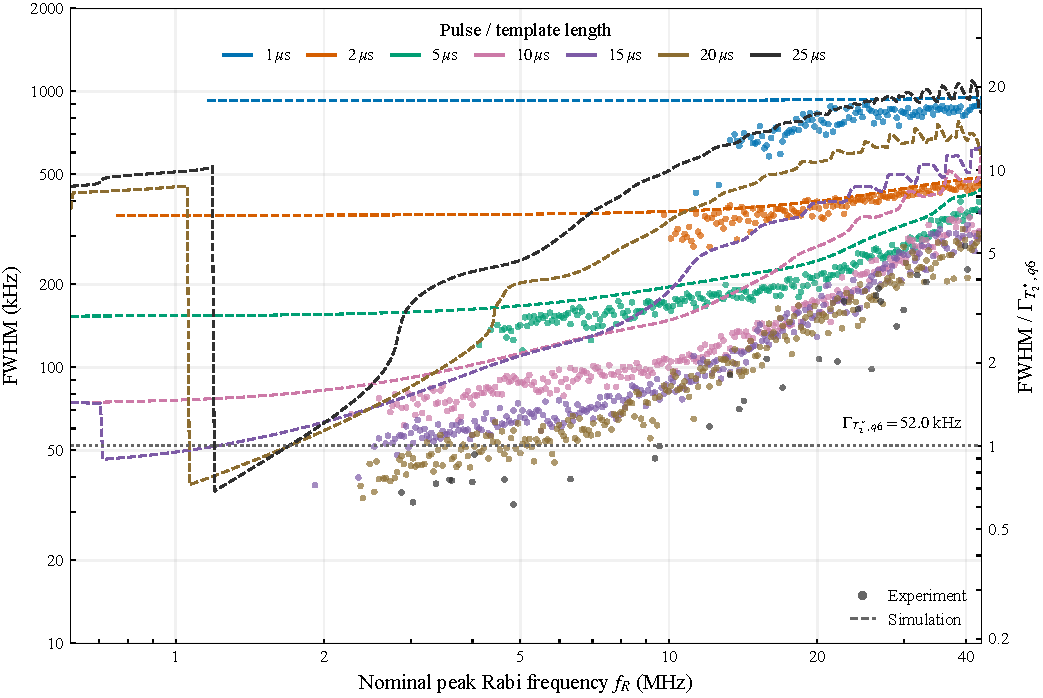
\includegraphics[width=\linewidth]{../figures/paper/12_pulse_length_linewidth.pdf}
    \caption{Pulse-length dependence at $c=0.005$, $\beta=0$, and effective
    $\kappa=0$. Dots are accepted experimental FWHM values and dashed
    curves are simulated widths; color identifies the common pulse and
    template duration. The horizontal axis is the calibrated nominal peak
    Rabi frequency $f_R=\Omega_0/(2\pi)$. Both axes are logarithmic.
    The right axis divides the linewidth by the campaign-specific
    $\Gamma_{T_2^*,q6}=51.996~\mathrm{kHz}$; the dotted line marks unity.
    Only accepted widths are shown, without additional smoothing or
    averaging across durations.}
    \label{fig:dense-pulse-length-widths}
\end{figure}

Figure~\ref{fig:dense-paired-linewidths} compares widths at the same
acquired amplitude index and duration, using the intersection of the two
acceptance masks. There are 1278 pairs in total, with counts of
110, 135, 213, 260, 265, 263 and 32 for the seven increasing durations.
At $2~\mu\mathrm{s}$ the paired linewidth RMS difference is
$34.2~\mathrm{kHz}$; it increases to $302.5~\mathrm{kHz}$ at
$20~\mu\mathrm{s}$. Most long-duration pairs fall below the equality
line: the simulation predicts broader features than the experiment.
Pairing accepted widths does not by itself establish that the strongest
feature selected in each trace has the same physical origin.

\begin{figure}[htbp]
    \centering
    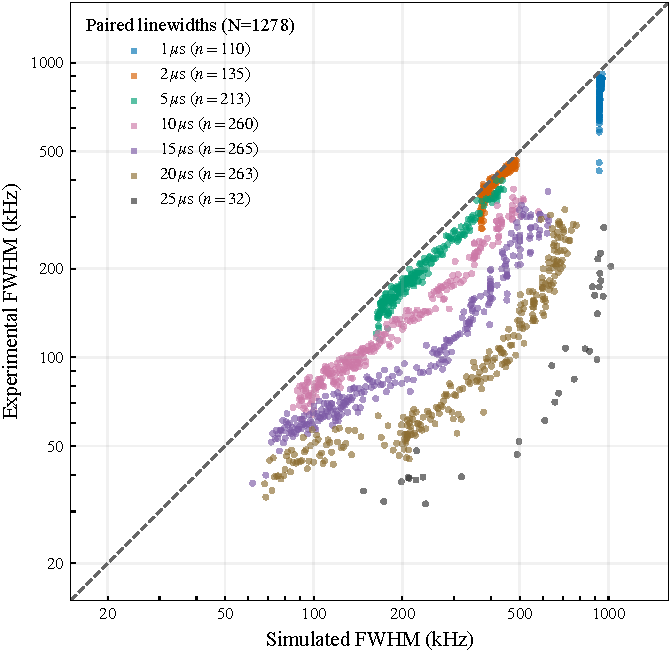
\includegraphics[width=0.79\linewidth]{../figures/paper/12_pulse_length_paired_linewidths.pdf}
    \caption{Paired experimental and simulated FWHM for the same seven
    durations and color convention as
    Fig.~\ref{fig:dense-pulse-length-widths}. Each point uses the same
    duration and nominal drive setting in both datasets, and both widths
    must pass their respective selection rules. Legend counts give the
    accepted pairs per duration. The dashed diagonal denotes equality;
    points below it have a narrower experimental than simulated feature.
    No linewidth uncertainty bars are assigned.}
    \label{fig:dense-paired-linewidths}
\end{figure}

Only 32 of 400 experimental traces pass the selection at
$25~\mu\mathrm{s}$, and none do so at $30$, $35$ or $40~\mu\mathrm{s}$.
These missing widths mean that the feature is not reliably resolved by
this estimator, rather than that its linewidth vanishes. The surviving
sets therefore differ across durations; the longer-duration comparison
is conditional on the small accepted subset. Because the maps were
acquired sequentially over approximately 8.6 hours without repeated
campaigns, drift and pulse-length effects are not independently separated.
The data support a duration-dependent narrowing and loss of measurable
contrast, but do not establish an optimal duration or a universal
coherence-limited plateau.
\FloatBarrier
